%=============================================================================
% Denoising Chapter
% Copyright (c) 2018. Lester James V. Miranda
%
% This file is part of thesis-manuscript.
%
% thesis-manuscript is free software: you can redistribute it and/or modify
% it under the terms of the GNU General Public License as published by
% the Free Software Foundation, either version 3 of the License, or
% (at your option) any later version.
%
% thesis-manuscript is distributed in the hope that it will be useful,
% but WITHOUT ANY WARRANTY; without even the implied warranty of
% MERCHANTABILITY or FITNESS FOR A PARTICULAR PURPOSE.  See the
% GNU General Public License for more details.
%
% You should have received a copy of the GNU General Public License
% along with thesis-manuscript.  If not, see <http://www.gnu.org/licenses/>.
%
% Created by: Lester James V. Miranda <ljvmiranda@gmail.com>
%=============================================================================

\chapter[Stacked Denoising Autoencoder for Protein Function Prediction]{
    \huge
    Feature Extraction using a Stacked Denoising Autoencoder for Protein
    Function Prediction
}
\label{SDAEChapter}

\par This chapter describes preliminary work where we extracted robust
features using a stacked denoising autoencoder (SdAE). Our main contribution
is that we have demonstrated the effectiveness of extracting features via
SdAE, commonly-used in images, in multilabel protein datasets. We start by
describing the SdAE architecture (Sec. \ref{SDArchitecture}), then illustrate
how it fits in the protein function prediction pipeline (Sec.
\ref{SDPipeline}). Then, we describe our experimental set-up (Sec.
\ref{SDSetup}), present our findings (Sec. \ref{SDResults}), and draw conclusions
(Sec. \ref{SDConclusions}).

\section{Stacked Denoising Autoencoder}
\label{SDArchitecture}

\begin{wrapfigure}{r}{0.53\textwidth}
  \centering
  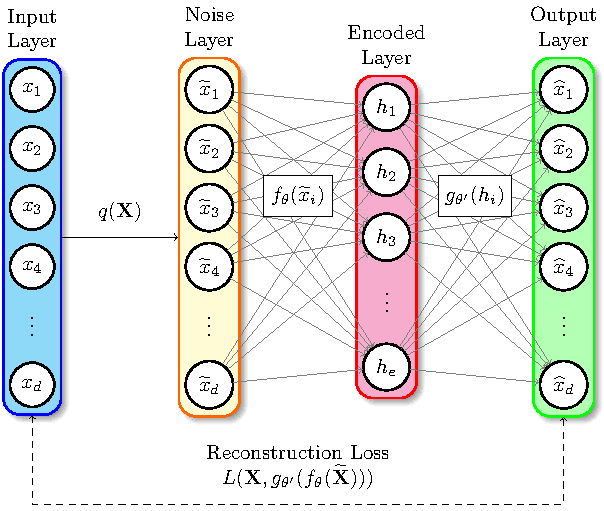
\includegraphics[width=0.5\textwidth]{ch03/sdae}
  \caption{Stacked denoising autoencoder}
  \label{schema:sdae}
\end{wrapfigure}

\par A stacked denoising autoencoder (SdAE) is a type of autoencoder that
corrupts the input data before reconstruction (\cite{vincent2010stacked}). It
is an extension of denoising autoencoders where layers are stacked and
greedily-trained\footnote{Greedy layer-wise training were once implemented
for practicality and to conserve memory (\cite{bengio2007greedy}). Today,
deep autoencoders like SdAE are trained end-to-end.}
(\cite{vincent2008denoising}).

\par Figure \ref{schema:sdae} illustrates the SdAE architecture. Given an
input data $\mathbf{X}$, we apply a corrupting function
$q(\mathcal{X}=\mathbf{X})$ to obtain a set of \textit{corrupted inputs}
$\mathbf{\widetilde{X}}$. We use the corrupted input to train the
autoencoder, but we compute the reconstruction loss by comparing the
reconstructed features $\mathbf{\widehat{X}}$ with the original data
$\mathbf{X}$. By learning from a set of corrupted inputs, we can capture the
``main factors of variations in the data (\cite{vincent2008denoising}),''
enabling our model to generalize unseen instances in the problem domain.
In theory, this should improve classification performance.

\subsection{More on generalization and manifold learning}

\begin{wrapfigure}{r}{0.5\textwidth}
  \centering
  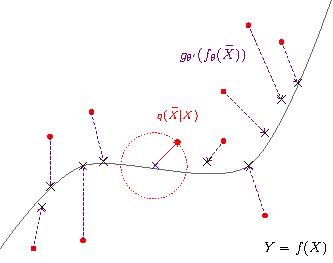
\includegraphics[width=0.45\textwidth]{ch03/demo_manifold}
  \caption[Manifold demonstration in SdAE]{Manifold learning in SdAE. Adapted
  from \cite{vincent2008denoising}}
  \label{demo:manifold}
\end{wrapfigure}

\par We'll spend some time examining how a stacked denoising autoencoder's
corrupting function enables the model to generalize during training. Recall
that generalization prevents model overfitting, i.e. fitting too close to the
training set that results to poor performance on the test set. The test set
represents unseen or future instances and we want to perform well on that.
Thus, our goal is to obtain the main factors of variation from the samples.
Perceiving SdAEs this way permits us to transfer this method to a different
domain\textemdash in our case, multilabel protein data\textemdash with more
confidence.

\par Say we're given a training dataset $X$ (marked by $\times$) that lies on
a manifold represented by the spline in Figure \ref{demo:manifold}. In
practice, we don't know what the spline looks like and the training data is
not always perfect.\footnote{
  The training data will not always be lying on-top of the spline. We know
  this to be true because there will always be unmodeled physics or
  measurement errors (i.e., $x+\epsilon$) that we cannot always account
  during data acquisition.
} Our task is to learn the manifold equivalent to identifying the structure
of the spline. Applying the noise function $q(\widetilde{X}|X)$ results to
data points $\widetilde{x}$ (red dots) that are further away from the spline.
SdAE learns the manifold by projecting the noisy inputs back as demonstrated
by the dotted lines $g_{\theta^{\prime}}(f_{\theta}(\widetilde{X}))$
(\cite{vincent2008denoising}). As shown, the projections can approximate the
manifold and accommodate subtle variations even if a new data point is
slightly-off the spline. This idea is crucial given the pretext that protein
datasets are inherently noisy due to unaccounted measurement errors (Sec.
\ref{ProteinFunctionPrediction}).

\begin{figure}[h]
  \centering
  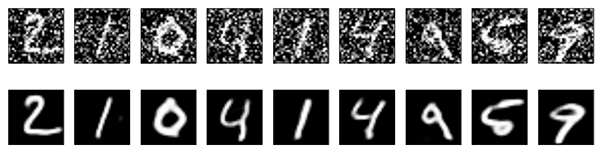
\includegraphics[width=0.9\textwidth]{ch03/demo_denoise}
  \caption[Demonstration of image denoising via SdAE]{
    Demonstration of image denoising via SdAE (\cite{chollet2016autoencoders})}
  \label{demo:denoise}
\end{figure}

\par Figure \ref{demo:denoise} demonstrates the reconstruction capability of
SdAE in the MNIST dataset. It has learned to ``ignore'' the unnecessary
variations in the data (noise) while focusing on the structural manifold of
the image. As a result, it was able to reproduce cleaner images from noisy
samples. It is evident that SdAE has learned to distinguish between relevant
and irrelevant aspects of the image: it retained useful information (the
actual digit) while discarding unnecessary ones (random noise).

\subsection{Practical considerations for SdAE training}

\par Table \ref{exp:noise_types} describes three different corrupting functions
for SdAE. We applied the salt-and-pepper (SP) noise for the dataset has been
preprocessed by normalizing the inputs in the $\left[0,1\right]$ range. It is
also a natural choice due to the hidden representations being squashed by a
sigmoid function.

\begin{table}[!h]
  \centering
  \caption[Different types of corrupting functions $q(\mathcal{X}) for SdAE$]
  {Different types of corrupting functions $q(\mathcal{X})$ for SdAE\\
  (\cite{vincent2010stacked})}
  \label{exp:noise_types}
  \begin{tabular}{@{}rp{0.70\textwidth}@{}}
      \toprule
      Noise            & Description                                                   \\ \midrule
      Gaussian         & additive isotropic Gaussian noise $\mathbf{\widetilde{x}} |
                         \mathbf{x} \sim \mathcal{N}(\mathbf{x}, \sigma^2 I)$          \\
      Masking          & a random sample of elements in $\mathbf{x}$ are forced to $0$ \\
      Salt-and-Pepper  & a random sample of elements in $\mathbf{x}$ is set to their
                         maximum or minimum value (usually $0$ or $1$)                 \\\bottomrule
  \end{tabular}
\end{table}

\par We introduce a hyperparameter, noise rate ($r$), that dictates how much of
the elements in $\mathbf{x}$ will be affected by the noise. For
salt-and-pepper, this determines the percentage of features, that will be set
to $0$ or $1$ based on a coin flip i.e., $P(0) = P(1) = 0.5$.


\par Lastly, Algorithm \ref{algo:sdae} describes the training procedure for SdAE.
It is similar to a deep autoencoder (Alg. \ref{algo:autoenc}), where the only difference
is that we corrupt the inputs first. In the next section, we will present how
we incorporated SdAE in the protein function prediction pipeline.

%=============================================================================
% algo_sdae.tex
% Copyright (c) 2018. Lester James V. Miranda
%
% This file is part of thesis-manuscript.
%
% thesis-mansucript is free software: you can redistribute it and/or modify
% it under the terms of the GNU General Public License as published by
% the Free Software Foundation, either version 3 of the License, or
% (at your option) any later version.
%
% thesis-manuscript is distributed in the hope that it will be useful,
% but WITHOUT ANY WARRANTY; without even the implied warranty of
% MERCHANTABILITY or FITNESS FOR A PARTICULAR PURPOSE.  See the
% GNU General Public License for more details.
%
% You should have received a copy of the GNU General Public License
% along with thesis-manuscript.  If not, see <http://www.gnu.org/licenses/>.
%
% Created by: Lester James V. Miranda <ljvmiranda@gmail.com>
%=============================================================================

\begin{algorithm}
    \caption{Training a stacked denoising autoencoder}
    \label{algo:sdae}
    \begin{algorithmic}[1]
    
    \INPUT Raw attributes $\mathbf{X}$, Noise rate $r$
    \OUTPUT Learned parameters $\theta^{\ast}$

    \item[]
    \State $\mathbf{\widetilde{X}} \gets q(\mathbf{X}, r)$
    \Comment Corrupt inputs
    \For{\textit{NumEpochs}}
        \State $\mathbf{h} \gets f_{\theta}(\mathbf{\widetilde{X}}) = \sigma(\theta\mathbf{\widetilde{X}}^{T} + \theta_0)$
        \Comment Encoder function
        \State $\mathbf{\widehat{X}} \gets g_{\theta^{\prime}}(\mathbf{h}) = \sigma(\theta^{\prime} \mathbf{h}^{T} + \theta^{\prime}_{0})$
        \Comment Decoder with tied-weights, $\theta^{\prime}=\theta^{T}$
        \State $J(\theta) \gets L(\mathbf{X}, \mathbf{\widehat{X}})$
        \Comment Compute loss
        \State \Call{Backpropagation}{$J(\theta)$}
        \Comment Optimize parameters
    \EndFor
    \State \Return $\theta^{\ast}$
    \Comment Return learned parameters
    \end{algorithmic}
\end{algorithm}


\section{Protein Function Prediction Pipeline}
\label{SDPipeline}

\begin{figure}[!t]
  \centering
  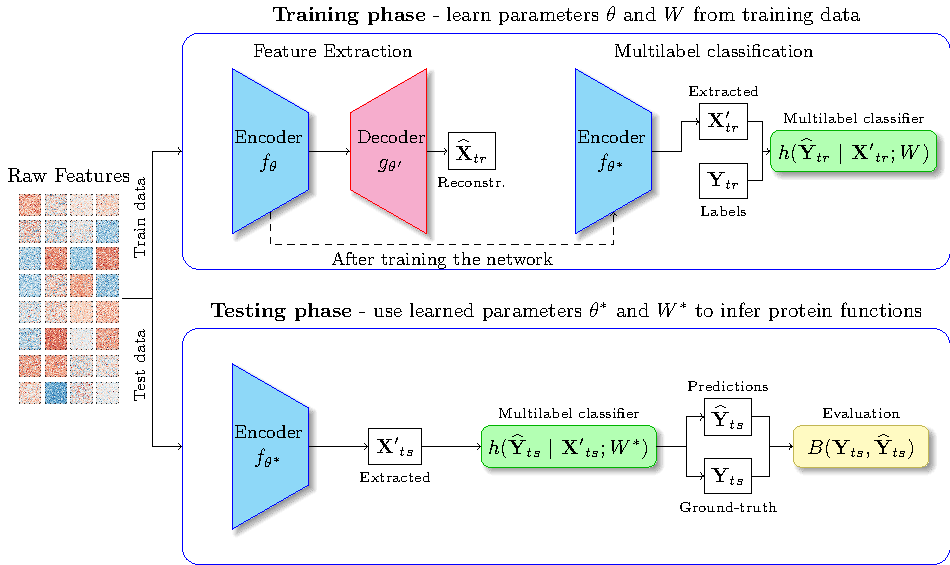
\includegraphics[width=0.90\textwidth]{ch03/schema_traintest}
  \caption[Protein function prediction pipeline]{Protein function prediction
  pipeline for the stacked denoising autoencoder}
  \label{schema:traintest_sdae}
\end{figure}

\par The protein function prediction pipeline consists of a (1) \textit{feature
extraction} and (2) \textit{multi-label classification} stage as shown in
Figure \ref{schema:traintest_sdae}.\footnote{
    Except for the corruption part, the pipeline in the mutually-competitive
    autoencoder (Chapter \ref{SelectiveChapter}) looks exactly like this.
} 
This follows the blueprint introduced in Figure \ref{schema:pipeline}: we have
a feature extractor $\phi$ that derives new features $X^{\prime}$ to train a
multilabel classifier $\mathcal{H}$. Here, the SdAE takes the role of the
feature extractor, and a binary-relevance support-vector machine (BR-SVM) as
the classifier. Our main goal is to find the best set of features $X^{\prime}$
that improves $\mathcal{H}$'s predictive performance. As with standard machine
learning practice, we have two phases\footnote{
  We usually split the dataset into training and test data such that
  $\mathcal{D} = \{\mathcal{D}_{tr}, \mathcal{D}_{ts}\}$. We didn't put the
  subscripts $tr$ and $ts$ for it can be easily inferred which set is being
  used in a given context.
}:

\begin{itemize}
  \item \textit{Training phase}: our goal is to learn the parameters $\theta$
  and $W$ for the extractor ($\phi$) and classifier ($\mathcal{H}$) stages
  respectively. We first train the SdAE using Alg. \ref{algo:sdae}, and use
  the learned $\theta^{\ast}$ to encode the training dataset for fitting
  BR-SVM. We use the mean-square error (MSE) as the loss-function for $\phi$ and
  L2-SVM for $\mathcal{H}$
  \begin{align}
    % Feature Extractor Loss
    \label{eqn:loss_fe_sdae}
    L(\mathbf{X},g_{\theta^{\prime}}(\mathbf{h}^{\prime})) &=
      \dfrac{1}{2}(\mathbf{X} - g_{\theta^{\prime}}(\mathbf{h}^{\prime}))^{2}\\
    % Multilabel classifier loss
    \label{eqn:loss_clf_sdae}
    J(\mathbf{X}^{\prime}, \widehat{\mathbf{Y}}, \mathbf{Y}) &= \sum_{\widehat{\mathbf{y}}_i \neq \mathbf{y}_{i}} \text{max}(0, W^{T}_{\widehat{\mathbf{y}}_{i}} \mathbf{x}_{i}^{\prime} - W^{T}_{\mathbf{y}_i}\mathbf{x}^{\prime}_i + \Delta)^2
  \end{align}
  \item \textit{Test phase}: this phase represents the scenario where we need
  to predict from unseen instances of protein data. We simply take the
  learned parameters $\{\theta^{\ast}, W^{\ast}\}$ and pass the test data
  through the encoder and classifier. The encoder derives new features given the
  equation: 
  \begin{align}
    % Encoder equation
    \label{eqn:encoder_mc_sdae}
    f_{\theta^{\ast}}(\mathbf{X}_{ts}) = \theta^{\ast T} \mathbf{X}_{ts} + \theta_{0}^{\ast}
  \end{align}
 
  \noindent Then the classifier infers from the derived features, producing a set of
  predictions $\mathbf{\widehat{Y}}_{ts}$. We compare our predictions to a
  held-out set of ground-truth labels using the metrics described in the next
  section.
\end{itemize}

\newpage
\subsection{Evaluation metrics}

To evaluate the performance of our prediction model, we will use the following
metrics\footnote[2]{\textit{tp}: true positive, \textit{fp}: false positive,
\textit{tn}: true negative, \textit{fn}: false negative}:

\begin{align}
    \text{Hamming Loss (H)} &= \dfrac{1}{N \cdot L} \sum_{i=1}^{N} \sum_{j=1}^{L}
    \text{XOR}(y_{ij}, \widehat{y}_{ij}) \\
    \text{Precision (P)} &=
    \dfrac{1}{N}\sum_{i=1}^{N}\dfrac{|\mathbf{\widehat{y}}_{i} \cap
    \mathbf{y}_{i}|}{|\mathbf{\widehat{y}_{i}}|} = \dfrac{tp}{tp + fp} \\
    \text{Recall (R)} &=
    \dfrac{1}{N}\sum_{i=1}^{N}\dfrac{|\mathbf{\widehat{y}}_{i} \cup
    \mathbf{y}_{i}|}{|\mathbf{\widehat{y}_{i}}|} = \dfrac{tp}{tp + fn} \\
    \text{F-score (F)} &=
    \dfrac{1}{N}\sum_{i=1}^{N} \dfrac{2 | \mathbf{\widehat{y}}_{i} \cup
        \mathbf{y}_{i}|}{|\mathbf{\widehat{y}}_{i} | + |\mathbf{y}_{i}|} =
        \dfrac{2 (\text{P} \cdot \text{R})}{\text{P} +
        \text{R}}
\end{align}

\par We will also compute for a fifth metric, the Area Under the ROC Curve
(AUROC), to serve as proxy for accuracy. For benchmarking, we will use the AUROC,
Hamming-Loss and F-score. Note that these metrics will exactly be the same for
our work on mutually-competitive autoencoders in Chapter \ref{SelectiveChapter}.

\section{Experimental Set-up}
\label{SDSetup}

\par We performed two (2) sets of experiments for the SdAE-based protein
function prediction pipeline. First, we checked how each hyperparameter,
i.e., noise rate ($r$) and number of encoding units ($e$), affects a
classifier's predictive performance. Then, we benchmarked our model against
different techniques in literature. Table \ref{exp:setup_sdae}
shows a summary of all experiments conducted in this work.

\begin{table}[h]
  \centering
  \caption{Summary of experiments}
  \label{exp:setup_sdae}
  \begin{threeparttable}
      \begin{tabular}{@{}rp{0.65\textwidth}@{}}
          \toprule
          Experiment & Description                                                            \\ \midrule
          \textit{Hyperparameter tests}                                                       \\
          Nb. of encoding units, $e$    & Test overcomplete and undercomplete configurations. \\
          Noise rate, $r$               & Sweep $k$-values in the range $\left[0,1\right]$    \\ \cmidrule{1-2} 
          \textit{Analysis \& benchmark}                                                      \\
          Model quality                 & Plot ROC and PR curves\tnote{1}                     \\
          Benchmark analysis            & Compare SdAE pipeline to other techniques\tnote{2}  \\ \bottomrule
      \end{tabular}
      \begin{tablenotes}
        \footnotesize
        \item[1] ROC - Receiver Operating Characteristic, PR - Precision--Recall
        \item[2] Friedman's test \parencite{friedman1937use} and post-hoc
        Bonferroni-Holm test \parencite{holm1979simple} were employed to
        measure statistical significance as recommended by
        \cite{demsar2006statistical}.
      \end{tablenotes}
    \end{threeparttable}
\end{table}

\par Lastly, Table \ref{exp:implementation_sdae} describes the experimental
environment for running the tests. The neural network was trained on an
NVIDIA Titan X (Pascal) GPU while the classifier was fitted using an Intel
Xeon 2.2GHz CPU. The majority of the code was written in Python 3.6.X using
the \href{https://www.tensorflow.org/}{Tensorflow} and
\href{https://keras.io/}{Keras} package. 

\begin{table}[t]
  \centering
  \caption{Experimental environment}
  \label{exp:implementation_sdae}
  \begin{threeparttable}
  \begin{tabular}{@{}rp{0.70\textwidth}@{}}
      \toprule
      Environment                    & Value                                             \\ \midrule
      \textit{Validation and testing}                                                    \\
      Number of trials               & 10: mean and std. dev. reported                   \\
      Train--validation--test split  & 50--30--20                                        \\ \cmidrule{1-2}
      \textit{Hardware dependencies}                                                     \\
      Number of cores\tnote{1}       & 10 in use (40 maximum)                            \\
      CPU                            & Intel Xeon 2.2GHz: Classifier training            \\
      GPU                            & NVIDIA Titan X (PASCAL): Neural network training  \\ \cmidrule{1-2} 
      \textit{Software dependencies}                                                     \\
      Language                & Python 2.7, 3.6 (compatible to both versions)            \\
      Libraries               & Tensorflow 1.2.1, Keras 2.1.2, Numpy 1.14.2              \\ \bottomrule
  \end{tabular}
  \begin{tablenotes}
    \footnotesize
    \item[1] We implemented a distributed scheme for training the classifier.
    Please see Appendix \ref{AppendixDistributed}.
  \end{tablenotes}
  \end{threeparttable}
\end{table}

\section{Results and Discussion}
\label{SDResults}

In this section, we'll present the results listed in Table
\ref{exp:setup_sdae}. First, we'll look into how different hyperparameter
settings\textemdash namely, noise rate ($r$) and number of encoding units
($e$)\textemdash affects the model as a whole. Then, we'll inspect the
quality of our model, and compare it with various works in literature.
For implementation details, please see \ref{AppendixImplementation}.

\subsection{Characterizing the autoencoder model}

Our goal in this experiment is to find a pattern governing model behavior
with respect to different hyperparameter values. The idea is to take a
hyperparameter $\mathcal{P}$ and change its value while measuring the Area
under the ROC curve (AUROC). We then plot the results for both train and
validation data. We repeat this experiment for all datasets.

\subsubsection{Experiments on the Yeast Dataset}

Figure \ref{results:sdae_char_yeast} shows the characterization results for
Yeast. Recall that validation set performance should always be lower than
training set performance, as the former simulates unseen samples. Here we can
observe the following:

\begin{itemize}
  \item Undercomplete autoencoders perform well without much overfitting.
      Overfitting can be observed with higher values of $e$, exemplified by the
      large gap between training and validation set performance; the model can
      predict the training data well, but fails to accommodate unseen instances
      of the validation data.
  \item Adding noise is beneficial, but too much noise can damage the model.
      Noise provides a good generalization ability to the model, and this
      confirms the ideas presented in denoising autoencoder literature
      (\cite{vincent2008denoising, vincent2010stacked}).
\end{itemize}
 
\begin{figure}[!t]
  \centering
  \begin{subfigure}[b]{0.48\textwidth}
    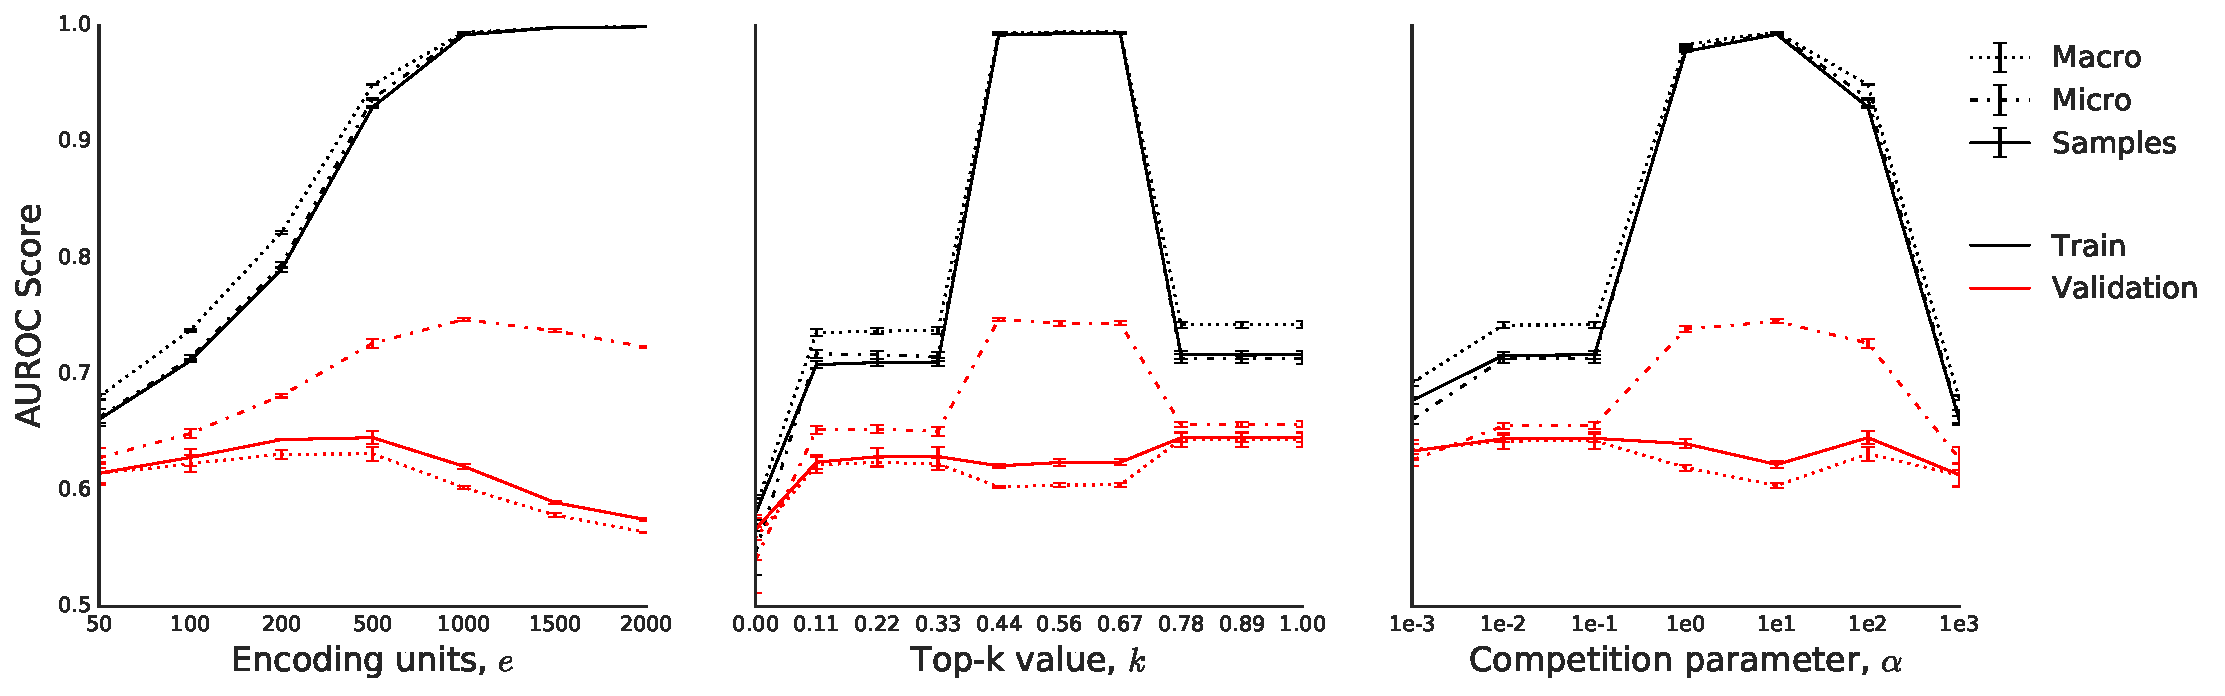
\includegraphics[width=\textwidth]{ch03/hyperparams_yeast}
    \caption{Yeast}
    \label{results:sdae_char_yeast}
  \end{subfigure}
  \begin{subfigure}[b]{0.48\textwidth}
    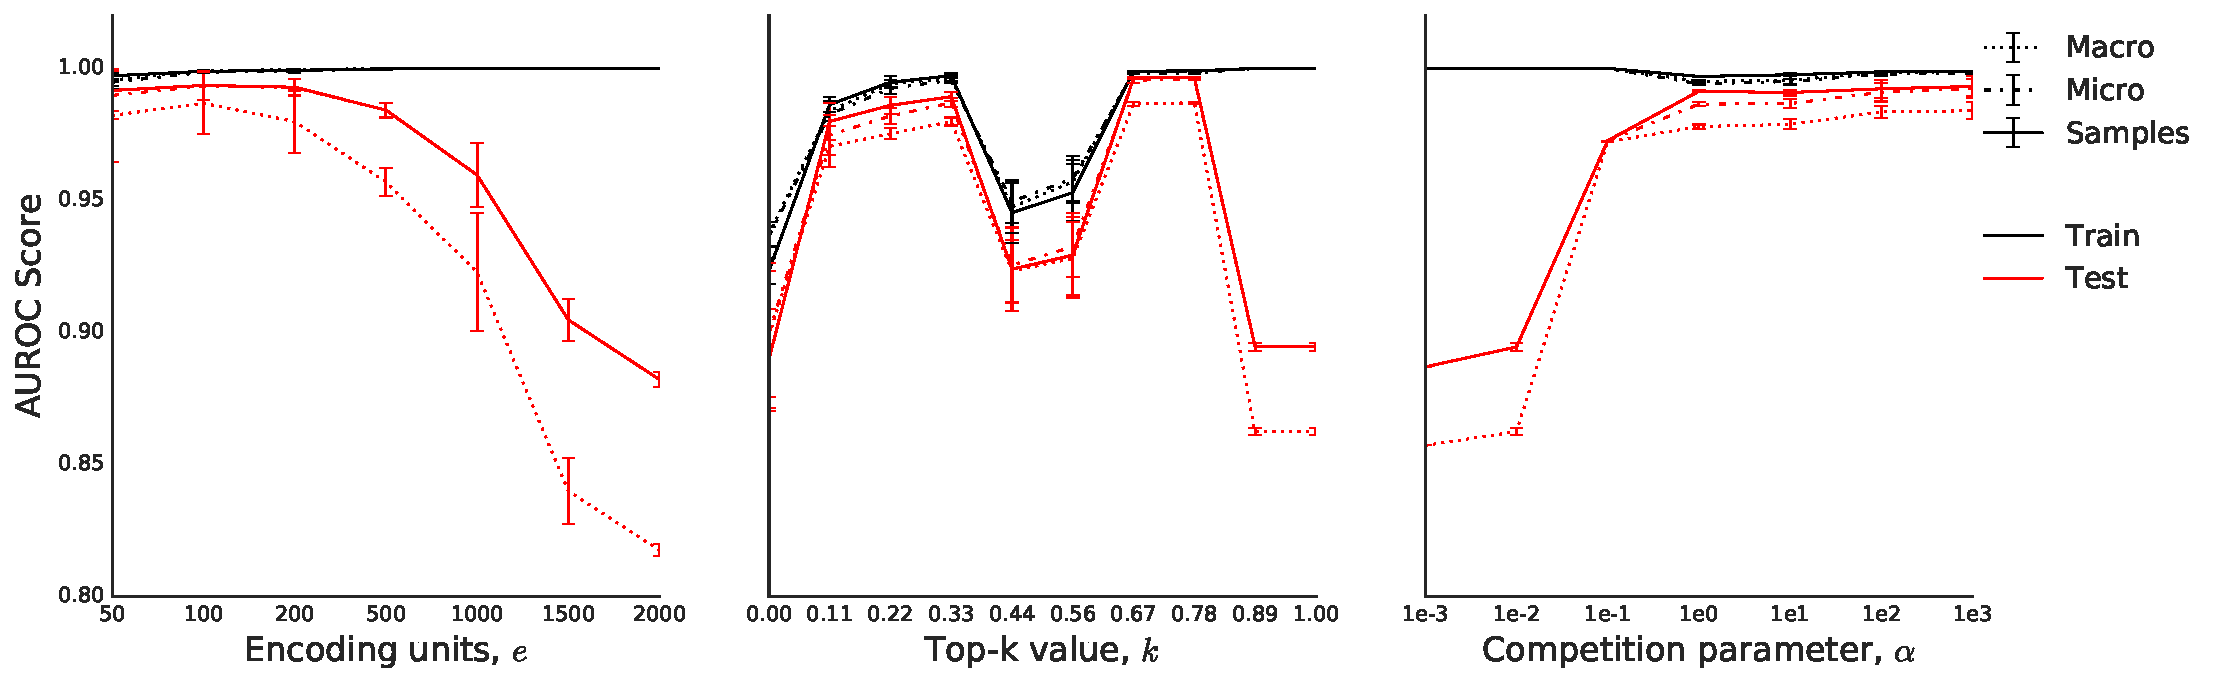
\includegraphics[width=\textwidth]{ch03/hyperparams_genbase}
    \caption{Genbase}
    \label{results:sdae_char_genbase}
  \end{subfigure}
  \caption{Model behavior on protein benchmarks}
  \label{results:sdae_char}
\end{figure}

\subsubsection{Experiments on the Genbase Dataset}

Figure \ref{results:sdae_char_genbase} shows the results for Genbase. A similar
procedure was performed for both training and validation data. We can infer
the following from the plots:

\begin{itemize}
  \item SdAE performance on Genbase is good overall. The small gap between
      training and validation performance shows that the model can perform well
      even with unseen instances of the data.
  \item Adding noise is also beneficial, but, similar to Yeast, may lead to
      overfitting if too much. Notice that validation performance is flat, this
      is due to the network having a smaller number of encoding units and
      shorter training time in this set-up ($e=50$ and $\text{epochs}=100$).
\end{itemize}

\subsection{Key results for the stacked denoising autoencoder}

In this section, we present our key results for the stacked denoising
autoencoder. First, we plot model quality in terms of the Receiver Operating
Characteristic (ROC) and Precision-Recall curves, then we present
benchmarking results against different models. Unlike the previous
experiment, we'll be reporting test set performance instead of the validation
set.

\subsubsection{Assessing model quality}

\par The goal of this experiment is to check if the SdAE-based pipeline can
indeed predict protein functions effectively. We can achieve this by plotting
the Receiver Operating Characteristic (ROC) and Precision-Recall (PR) curves
for both datasets and interpreting their shapes. 

\begin{figure}[!h]
  \centering
  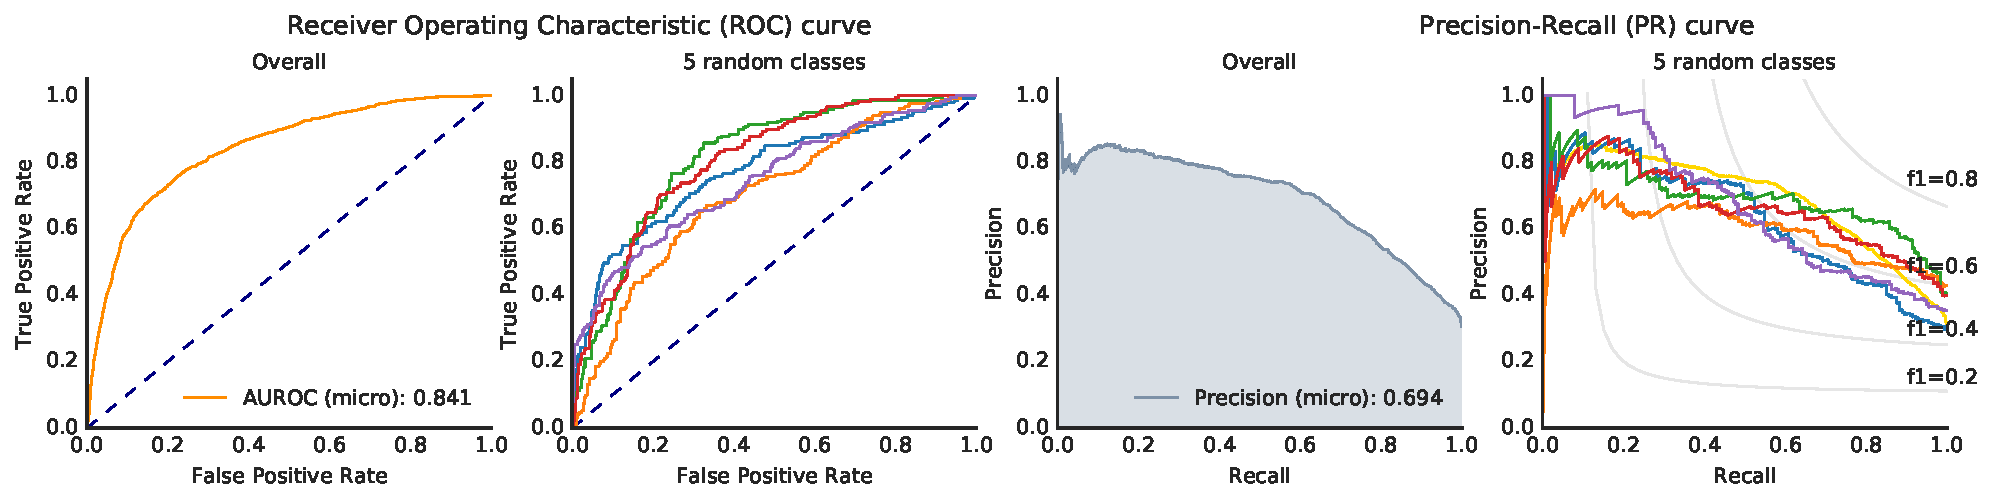
\includegraphics[width=0.95\textwidth]{ch03/ql_yeast}
  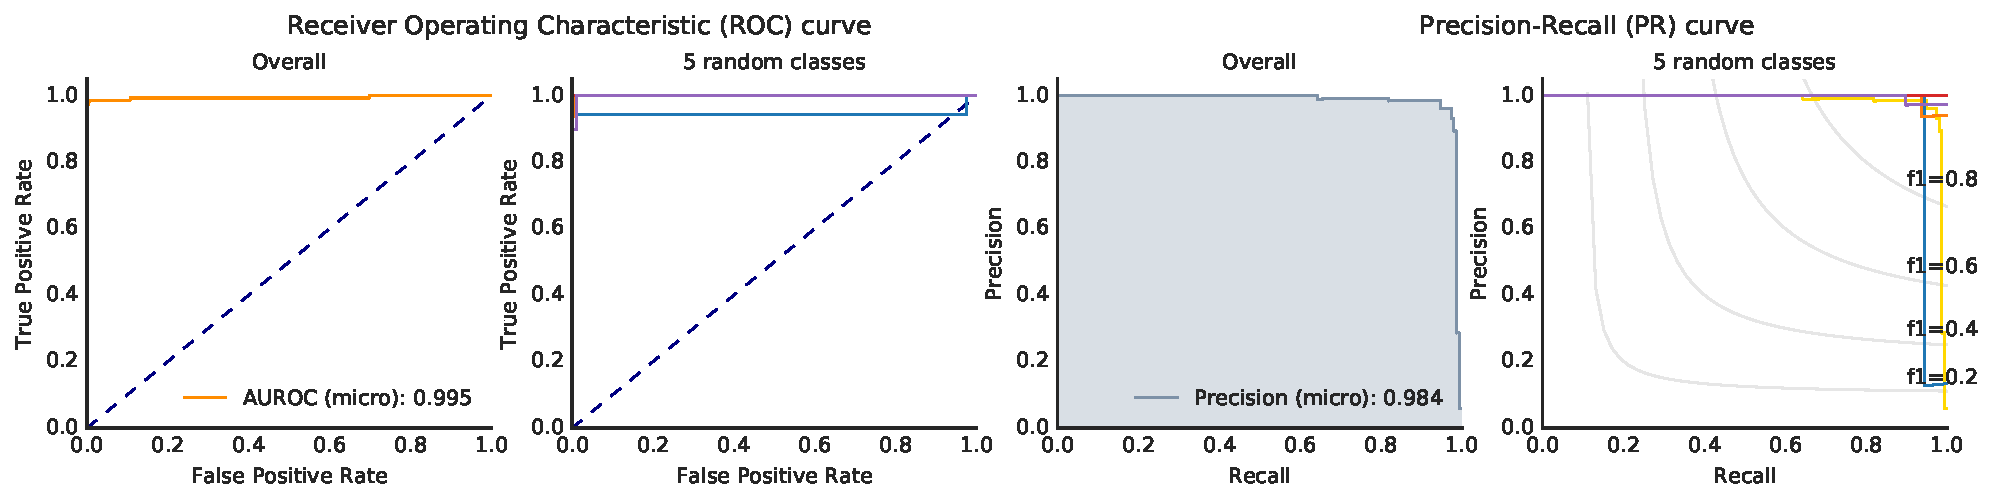
\includegraphics[width=0.95\textwidth]{ch03/ql_genbase}
  \caption[Receiver Operating Characteristic (ROC) and Precision-Recall (PR)
  curves for the two protein benchmarks]{
    Receiver Operating Characteristic (ROC) and Precision-Recall (PR) curves
    for both Yeast (\textit{top}) and Genbase (\textit{bottom}) datasets.
  }
  \label{results:sdae_quality}
\end{figure}


\par A good indicator of quality for an ROC curve is to check how far the
orange line, representing the FPR and TPR at different cutoff points, is from
the baseline (representing a random classifier). It is apparent that for both
datasets, the curve is way above the baseline\textemdash and moreso with
Genbase. In addition, measuring the AUROC gives a good predictive accuracy.
On the other hand, Precision-Recall curves show the tradeoff between
precision and recall for both datasets. It is apparent that Genbase has a
consistently high precision, whereas Yeast has decent quality. In the next
experiment, we'll put our prediction pipeline into context by comparing it
with other works in literature.


\subsection{Benchmark analysis}

\par In this experiment, we will compare against various protein function
prediction models in literature. The AUROC, F-score, and Hamming Loss will
measure model performance for both datasets. The results can be seen in
Tables \ref{results:sdae_benchmark_yeast} and
\ref{results:sdae_benchmark_genbase}

\par In addition, we conducted Friedman's test to assess significance in our
measurements. The null hypothesis $H_{0}$ dictates that there is no
significant difference between the groups. The ``Sig.'' column indicates the
extent in $\alpha$ in which we can reject $H_{0}$. The intuition is: the more
stars, the more confidence in the differences of the results.

\par For most metrics, the SdAE-based prediction pipeline performs well.
However, it is interesting that PCA (M1) and AE (M2) -based models have a
better AUROC performance. This can be attributed to some models having high
numbers of false negatives in their predictions, thus resulting to higher
accuracy given sparse labelsets. In fact, it may be easier to get high accuracy
by just predicting all samples as a zero-vector because of label sparsity.
However, if we look into the F-score metric, our model's predictive ability
becomes more apparent. Its high F-score suggests that our prediction pipeline
can better balance between precision and recall (false positives and false
negatives). Lastly, an overall comparison using a post-hoc Bonferroni-Holm test
shows that our SdAE-based model outperforms other models, especially the
baseline. Outperforming the baseline is critical because it validates our claim
that using feature extraction is beneficial to multilabel classification.

\begin{table}[!t]
%
\centering
\begin{threeparttable}
\caption{Benchmark analysis on Yeast dataset}
\label{results:sdae_benchmark_yeast}
%
\begin{tabular}{@{}rr*{5}{l}@{}}
\toprule
        & & \multicolumn{5}{c}{Prediction Model\tnote{1}} \\ \cmidrule{3-6}
Metrics & Avg.      & Baseline       & M1             & M2                 & Proposed\tnote{2} & Sig.\tnote{3}\\
\midrule
AUROC   & micro     & \num{0.667(3)} & \num{0.666(2)} & \num{0.643(1)}     & \hg\num{0.668(4)}  & *** \\
        & macro     & \num{0.655(3)} & \num{0.659(2)} & \hg \num{0.662(1)} & \num{0.648(2)}     & *** \\
        & sample    & \hg\num{0.670(3)} & \num{0.656(2)} & \num{0.643(1)}  & \num{0.657(3)}     & *** \\
F-score & micro     & \num{0.548(4)} & \num{0.538(2)} & \num{0.530(1)}     & \hg\num{0.579(3)}  & *** \\
        & macro     & \num{0.597(4)} & \num{0.603(2)} & \num{0.590(1)}     & \hg\num{0.613(2)}  & *** \\
        & sample    & \num{0.536(3)} & \num{0.524(2)} & \num{0.517(1)}     & \hg\num{0.572(3)}  & *** \\
Hamming Loss & --   & \num{0.322(2)} & \num{0.343(2)} & \num{0.354(1)}     & \hg \num{0.231(3)} & *** \\
\bottomrule
\end{tabular}
%
\begin{tablenotes}
        \footnotesize
    \item[1] M1: \cite{wang2013protein}, M2: \cite{chicco2014deep}
    \item[2] Feature ext.: $\{r=0.75,e=103-100-80\}$, BR-SVM: $\{C=\num{1.00}, \gamma=\num{1.292e-2}\}$
    \item[3] Significance: *-$p\leq 0.1$, **-$p\leq 0.05$, ***-$p\leq 0.01$
\end{tablenotes}
%
\end{threeparttable}
%
\end{table}


\begin{table}[!t]
%
\centering
\begin{threeparttable}
\caption{Benchmark analysis on Genbase dataset}
\label{results:sdae_benchmark_genbase}
%
\begin{tabular}{@{}rrlllll@{}}
\toprule
        &        &  \multicolumn{5}{c}{Prediction Model\tnote{1}} \\ \cmidrule{3-6}
Metrics & Avg.   & Baseline       & M1             & M2             & Proposed\tnote{2}   & Sig.\tnote{3}\\
\midrule
AUROC   & micro  & \num{0.856(0)} & \hg\num{0.987(0)} & \num{0.974(10)} & \hg\num{0.987(1)}     & ***  \\
        & macro  & \num{0.671(0)} & \hg\num{0.992(0)} & \num{0.979(11)} & \num{0.983(1)}        & ***  \\
        & sample & \num{0.613(0)} & \num{0.950(0)}    & \num{0.976(10)} & \hg\num{0.988(1)}     & ***  \\
F-score & micro  & \num{0.671(0)} & \num{0.887(1)}    & \num{0.785(87)} & \hg\num{0.962(11)}    & ***  \\
        & macro  & \num{0.716(0)} & \num{0.950(0)}    & \num{0.892(40)} & \hg\num{0.964(6)}     & ***  \\
        & sample & \num{0.760(0)} & \num{0.928(0)}    & \num{0.810(95)} & \hg\num{0.970(8)}     & ***  \\
Hamming Loss & -- & \num{0.041(0)} & \num{0.014(2)}   & \num{0.035(17)} & \hg\num{0.005(1)}     & ***  \\
\bottomrule
\end{tabular}
%
\begin{tablenotes}
    \footnotesize
    \item[*] Values with $0.XXX(0)$ stdev. have deviations in the ten-thousandths place 
    \item[1] M1: \cite{wang2013protein}, M2: \cite{chicco2014deep}
    \item[2] Feature ext.: $\{r=0.60, e=1186-50\}$, BR-SVM: $\{C=\num{1.668e2}, \gamma=\num{2.154e-4}\}$
    \item[3] Significance: *-$p\leq 0.1$, **-$p\leq 0.05$, ***-$p\leq 0.01$
\end{tablenotes}
%
\end{threeparttable}
%
\end{table}


\begin{table}[!h]
%
\centering
\begin{threeparttable}
\caption{One-vs-All Overall Comparison\\using post-hoc Bonferroni-Holm Test\tnote{1}}
\label{results:sdae_stats}
%
\begin{tabular}{@{}r*{3}{l}@{}}
\toprule
Proposed Model vs.                       & Z-statistic    & $p$-value         & Sig.\tnote{2} \\ \midrule
Baseline                                 & $3.373282$      & $0.00057$         & ***          \\
\cite{wang2013protein}                   & $3.440050$      & $0.00116$         & **           \\
\cite{chicco2014deep}                    & $1.903010$      & $0.05704$         & ***          \\ \bottomrule
\end{tabular}
\begin{tablenotes}
\footnotesize
\item[1] Friedman's test rejects $H_{0}$ with $\chi^{2}=\num{9.37050}$.
\item[2] Significance: *-$p\leq0.1$, **-$p\leq0.05$, ***-$p\leq0.01$
\end{tablenotes}
\end{threeparttable}
\end{table}



\newpage
\section{Conclusion}
\label{SDConclusions}

\par We explored the effectiveness of a stacked denoising autoencoder (SdAE),
commonly-used in images, in the domain of protein function prediction. By
adding small perturbations in the input and using it to train a network, we
can produce a model with high generalization ability. We tested this process
on two protein benchmarks, and evaluated the predictions using various
metrics.

\par By characterizing the model's response given different hyperparameter
values, we found out that an autoencoder's configuration greatly affects the
overall model's predictive performance. For SdAE, an undercomplete hidden
layer is beneficial. Too high a number can cause model overfitting: high
performance in the training set but low performance during validation. In
terms of noise rates, it turns out that adding perturbations can indeed
improve classification performance. However, this value is entirely dependent
on the dataset, and must be probed using search techniques.

\par Then, we plotted ROC and PR curves to check if the resulting SdAE-based
model can indeed predict protein functions. We found out that the model is
fairly accurate and in fact, has a good balance between precision and recall.
We put these findings into context by comparing against other techniques in
literature. Results show that the SdAE-based model outperforms other
techniques in most metrics, especially the F-score. The accuracy for other
models is high, but this can be attributed to high false negatives given
sparse labelsets. The SdAE-based model's high F-score confirms this
hypothesis. Lastly, it is important to mention that using extracted features
outperforms a Baseline model without feature extraction. This validates our
hypothesis that extracting features is crucial in predicting protein
functions.

\par This work demonstrates that using a stacked denoising autoencoder can
aid in predicting protein functions. Furthermore, we have successfully
transferred SdAE into another domain, i.e., multilabel protein data. By
corrupting the inputs, the autoencoder is ``forced'' to sift through the data
and determine which inputs are relevant or not. However, we have no control
on how these relevant inputs are determined. Instead, we just let the network
greedily obtain new features and trust that the resulting features are
relevant. It is then important to add a degree of control in determining
relevant features, without risking information loss. In the next chapter, we
will introduce the mutually-competitive autoencoder, a neural network
architecture we designed to extract relevant features while preserving
information from the dataset.
